\documentclass{standalone}
\usepackage{tikz}
\usetikzlibrary{patterns, positioning}


\begin{document}
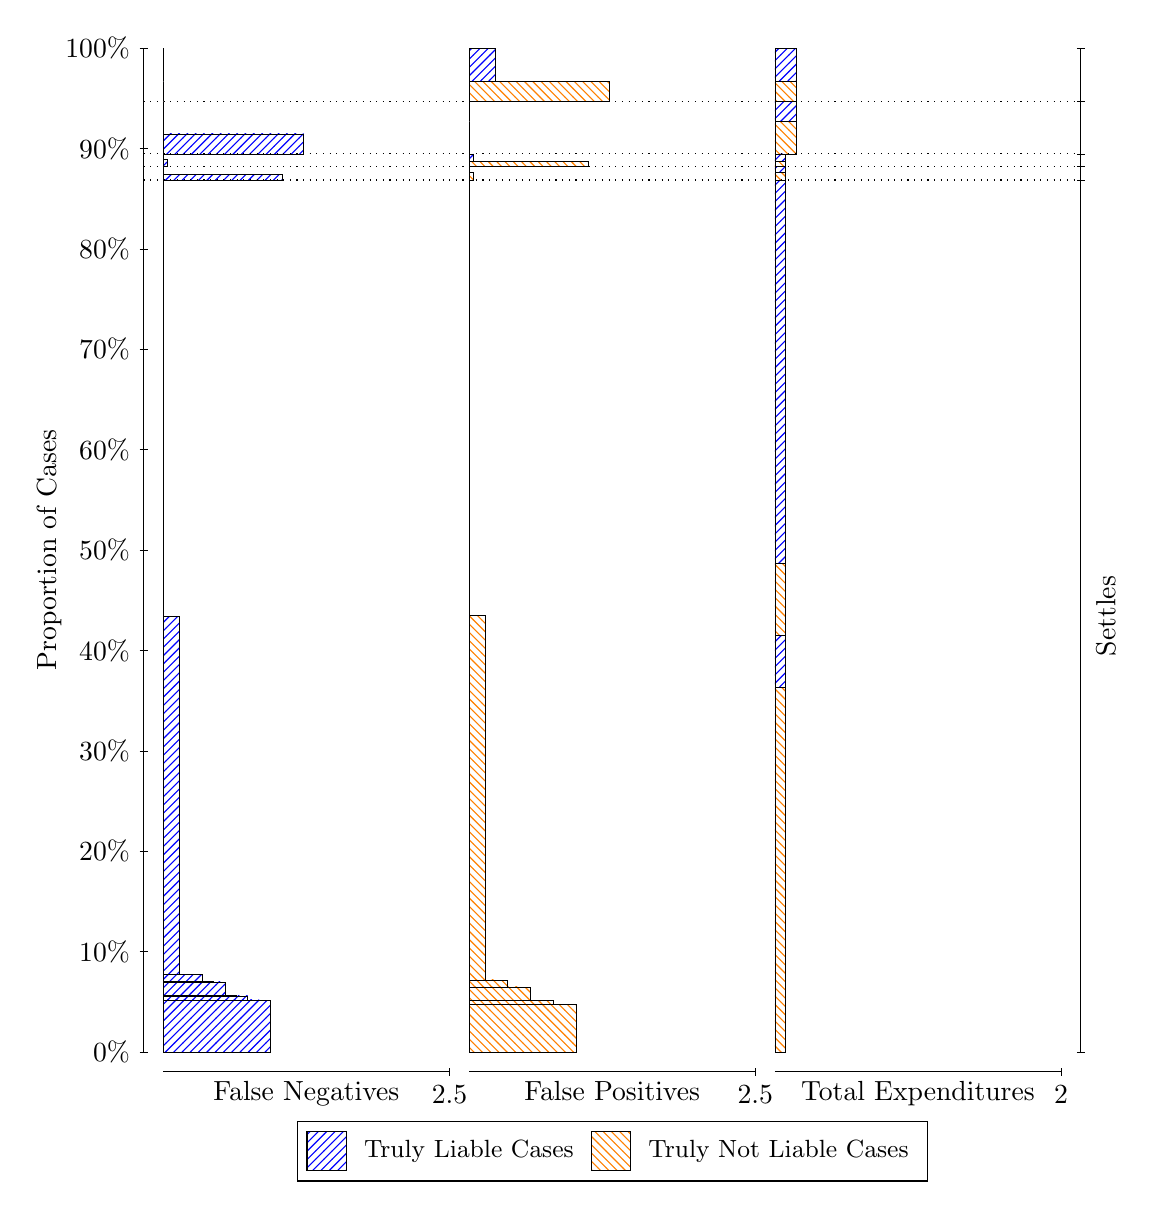
\begin{tikzpicture}
\draw[black, very thin] (1.5,1.75) -- (1.5,14.5);
\node[rotate=90, text=black, anchor=center] at (0.3, 8.125) {Proportion of Cases};
\draw[black, very thin] (1.45,1.75) -- (1.55,1.75);
\node[text=black, anchor=east] at (1.45, 1.75) {0\%};
\draw[black, very thin] (1.45,3.025) -- (1.55,3.025);
\node[text=black, anchor=east] at (1.45, 3.025) {10\%};
\draw[black, very thin] (1.45,4.3) -- (1.55,4.3);
\node[text=black, anchor=east] at (1.45, 4.3) {20\%};
\draw[black, very thin] (1.45,5.575) -- (1.55,5.575);
\node[text=black, anchor=east] at (1.45, 5.575) {30\%};
\draw[black, very thin] (1.45,6.85) -- (1.55,6.85);
\node[text=black, anchor=east] at (1.45, 6.85) {40\%};
\draw[black, very thin] (1.45,8.125) -- (1.55,8.125);
\node[text=black, anchor=east] at (1.45, 8.125) {50\%};
\draw[black, very thin] (1.45,9.4) -- (1.55,9.4);
\node[text=black, anchor=east] at (1.45, 9.4) {60\%};
\draw[black, very thin] (1.45,10.675) -- (1.55,10.675);
\node[text=black, anchor=east] at (1.45, 10.675) {70\%};
\draw[black, very thin] (1.45,11.95) -- (1.55,11.95);
\node[text=black, anchor=east] at (1.45, 11.95) {80\%};
\draw[black, very thin] (1.45,13.225) -- (1.55,13.225);
\node[text=black, anchor=east] at (1.45, 13.225) {90\%};
\draw[black, very thin] (1.45,14.5) -- (1.55,14.5);
\node[text=black, anchor=east] at (1.45, 14.5) {100\%};

\draw[black, very thin] (13.4,1.75) -- (13.4,14.5);
\draw[black, very thin] (13.35,1.75) -- (13.45,1.75);
\node[anchor=west] at (13.35, 1.75) {};
\draw[black, very thin] (13.35,12.824) -- (13.45,12.824);
\node[anchor=west] at (13.35, 12.824) {};
\draw[black, very thin] (13.35,12.992) -- (13.45,12.992);
\node[anchor=west] at (13.35, 12.992) {};
\draw[black, very thin] (13.35,13.156) -- (13.45,13.156);
\node[anchor=west] at (13.35, 13.156) {};
\draw[black, very thin] (13.35,13.819) -- (13.45,13.819);
\node[anchor=west] at (13.35, 13.819) {};
\draw[black, very thin] (13.35,14.5) -- (13.45,14.5);
\node[anchor=west] at (13.35, 14.5) {};

\draw[black, very thin, pattern color=blue, pattern=north east lines] (1.75,1.75) rectangle (3.1125,2.4101);
\draw[black, very thin, pattern color=blue, pattern=north east lines] (1.75,2.4101) rectangle (2.9672,2.4126);
\draw[black, very thin, pattern color=blue, pattern=north east lines] (1.75,2.4126) rectangle (2.8218,2.462);
\draw[black, very thin, pattern color=blue, pattern=north east lines] (1.75,2.462) rectangle (2.6765,2.4655);
\draw[black, very thin, pattern color=blue, pattern=north east lines] (1.75,2.4655) rectangle (2.5312,2.6391);
\draw[black, very thin, pattern color=blue, pattern=north east lines] (1.75,2.6391) rectangle (2.3858,2.6447);
\draw[black, very thin, pattern color=blue, pattern=north east lines] (1.75,2.6447) rectangle (2.2405,2.7334);
\draw[black, very thin, pattern color=blue, pattern=north east lines] (1.75,2.7334) rectangle (2.0952,2.738);
\draw[black, very thin, pattern color=blue, pattern=north east lines] (1.75,2.738) rectangle (1.9498,7.2802);
\draw[black, very thin, pattern color=orange, pattern=north west lines] (1.75,7.2802) rectangle (1.75,12.824);
\draw[black, very thin, pattern color=blue, pattern=north east lines] (1.75,12.824) rectangle (3.2578,12.894);
\draw[black, very thin, pattern color=orange, pattern=north west lines] (1.75,12.894) rectangle (1.75,12.992);
\draw[black, very thin, pattern color=blue, pattern=north east lines] (1.75,12.992) rectangle (1.8045,13.088);
\draw[black, very thin, pattern color=orange, pattern=north west lines] (1.75,13.088) rectangle (1.75,13.156);
\draw[black, very thin, pattern color=blue, pattern=north east lines] (1.75,13.156) rectangle (3.5303,13.409);
\draw[black, very thin, pattern color=orange, pattern=north west lines] (1.75,13.409) rectangle (1.75,13.819);
\draw[black, very thin, pattern color=orange, pattern=north west lines] (1.75,13.819) rectangle (1.75,14.075);
\draw[black, very thin, pattern color=blue, pattern=north east lines] (1.75,14.075) rectangle (1.75,14.5);
\draw[black, very thin, pattern color=orange, pattern=north west lines] (5.6333,1.75) rectangle (6.9958,2.3559);
\draw[black, very thin, pattern color=orange, pattern=north west lines] (5.6333,2.3559) rectangle (6.8505,2.3584);
\draw[black, very thin, pattern color=orange, pattern=north west lines] (5.6333,2.3584) rectangle (6.7052,2.4064);
\draw[black, very thin, pattern color=orange, pattern=north west lines] (5.6333,2.4064) rectangle (6.5598,2.4098);
\draw[black, very thin, pattern color=orange, pattern=north west lines] (5.6333,2.4098) rectangle (6.4145,2.5701);
\draw[black, very thin, pattern color=orange, pattern=north west lines] (5.6333,2.5701) rectangle (6.2692,2.571);
\draw[black, very thin, pattern color=orange, pattern=north west lines] (5.6333,2.571) rectangle (6.2692,2.5754);
\draw[black, very thin, pattern color=orange, pattern=north west lines] (5.6333,2.5754) rectangle (6.1238,2.6617);
\draw[black, very thin, pattern color=orange, pattern=north west lines] (5.6333,2.6617) rectangle (5.9785,2.6661);
\draw[black, very thin, pattern color=orange, pattern=north west lines] (5.6333,2.6661) rectangle (5.8332,7.2934);
\draw[black, very thin, pattern color=blue, pattern=north east lines] (5.6333,7.2934) rectangle (5.6333,12.824);
\draw[black, very thin, pattern color=orange, pattern=north west lines] (5.6333,12.824) rectangle (5.6878,12.921);
\draw[black, very thin, pattern color=blue, pattern=north east lines] (5.6333,12.921) rectangle (5.6333,12.992);
\draw[black, very thin, pattern color=orange, pattern=north west lines] (5.6333,12.992) rectangle (7.1412,13.06);
\draw[black, very thin, pattern color=blue, pattern=north east lines] (5.6333,13.06) rectangle (5.6878,13.156);
\draw[black, very thin, pattern color=orange, pattern=north west lines] (5.6333,13.156) rectangle (5.6333,13.565);
\draw[black, very thin, pattern color=blue, pattern=north east lines] (5.6333,13.565) rectangle (5.6333,13.819);
\draw[black, very thin, pattern color=orange, pattern=north west lines] (5.6333,13.819) rectangle (7.4137,14.075);
\draw[black, very thin, pattern color=blue, pattern=north east lines] (5.6333,14.075) rectangle (5.9603,14.5);
\draw[black, very thin, pattern color=orange, pattern=north west lines] (9.5167,1.75) rectangle (9.6529,6.3817);
\draw[black, very thin, pattern color=blue, pattern=north east lines] (9.5167,6.3817) rectangle (9.6529,7.0443);
\draw[black, very thin, pattern color=orange, pattern=north west lines] (9.5167,7.0443) rectangle (9.6529,7.956);
\draw[black, very thin, pattern color=blue, pattern=north east lines] (9.5167,7.956) rectangle (9.6529,12.824);
\draw[black, very thin, pattern color=orange, pattern=north west lines] (9.5167,12.824) rectangle (9.6529,12.921);
\draw[black, very thin, pattern color=blue, pattern=north east lines] (9.5167,12.921) rectangle (9.6529,12.992);
\draw[black, very thin, pattern color=orange, pattern=north west lines] (9.5167,12.992) rectangle (9.6529,13.06);
\draw[black, very thin, pattern color=blue, pattern=north east lines] (9.5167,13.06) rectangle (9.6529,13.156);
\draw[black, very thin, pattern color=orange, pattern=north west lines] (9.5167,13.156) rectangle (9.7892,13.565);
\draw[black, very thin, pattern color=blue, pattern=north east lines] (9.5167,13.565) rectangle (9.7892,13.819);
\draw[black, very thin, pattern color=orange, pattern=north west lines] (9.5167,13.819) rectangle (9.7892,14.075);
\draw[black, very thin, pattern color=blue, pattern=north east lines] (9.5167,14.075) rectangle (9.7892,14.5);
\draw[black, dotted] (1.5,12.824) -- (13.4,12.824);
\draw[black, dotted] (1.5,12.992) -- (13.4,12.992);
\draw[black, dotted] (1.5,13.156) -- (13.4,13.156);
\draw[black, dotted] (1.5,13.819) -- (13.4,13.819);
\draw[black, very thin] (1.75,1.5) -- (5.3833,1.5);
\node[text=black, anchor=north] at (3.5667, 1.5) {False Negatives};
\draw[black, very thin] (5.3833,1.45) -- (5.3833,1.55);
\node[text=black, anchor=north] at (5.3833, 1.45) {2.5};

\draw[black, very thin] (5.6333,1.5) -- (9.2667,1.5);
\node[text=black, anchor=north] at (7.45, 1.5) {False Positives};
\draw[black, very thin] (9.2667,1.45) -- (9.2667,1.55);
\node[text=black, anchor=north] at (9.2667, 1.45) {2.5};

\draw[black, very thin] (9.5167,1.5) -- (13.15,1.5);
\node[text=black, anchor=north] at (11.333, 1.5) {Total Expenditures};
\draw[black, very thin] (13.15,1.45) -- (13.15,1.55);
\node[text=black, anchor=north] at (13.15, 1.45) {2};

\node[text=black, centered, rotate=90] at (13.72, 7.2868) {Settles};





\draw (7.449999999999999,1.5) node[draw=none] (baseCoordinate) {};
\begin{scope}[align=center]
        \matrix[scale=0.5, draw=black, below=0.5cm of baseCoordinate, nodes={draw}, column sep=0.1cm]{
            \node[rectangle, draw, minimum width=0.5cm, minimum height=0.5cm, pattern color=blue, pattern=north east lines] {}; &
            \node[draw=none, font=\small, text=black] (B) {Truly Liable Cases}; &
            \node[rectangle, draw, minimum width=0.5cm, minimum height=0.5cm, pattern color=orange, pattern=north west lines] {}; &
            \node[draw=none, font=\small, text=black] (B) {Truly Not Liable Cases}; \\
            };
\end{scope}

\end{tikzpicture}
\end{document}